\subsubsection{Die LEDs und ihre Bedeutungen}
\label{sec:leds}

Dieser Abschnitt erklärt die Bedeutung der LEDs.
Für diese Aufgabe war hauptsächlich Manuel Radatz verantwortlich, wobei die Bedeutungen der LEDs
auch im gesamten Team diskutiert worden sind.

\begin{figure}[h]
  \centering
  \begin{subfigure}[b]{0.22\textwidth}
    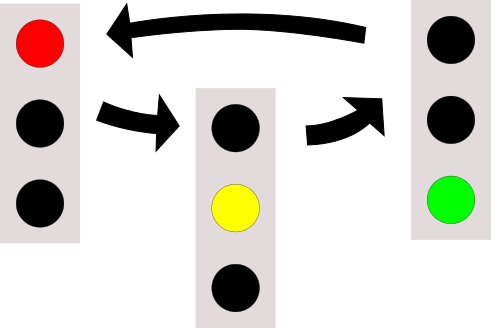
\includegraphics[width=\textwidth,keepaspectratio]
                    {./040-komponenten/010-hardware/led-default.png}
    \caption{\label{fig:led-init}}
  \end{subfigure}
  \hspace{0.1\textwidth}
  \begin{subfigure}[b]{0.40\textwidth}
    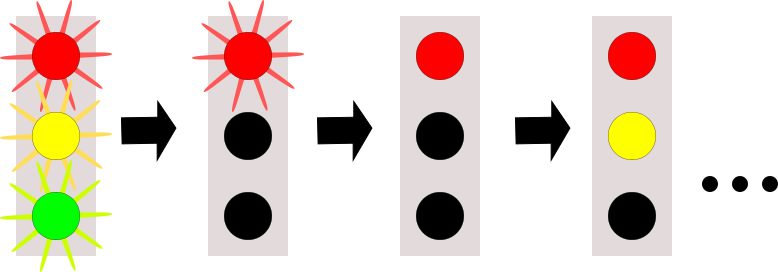
\includegraphics[width=\textwidth,keepaspectratio]{./040-komponenten/010-hardware/led-start.png}
    \caption{\label{fig:led-start}}
  \end{subfigure}
  
  \begin{subfigure}[b]{0.06\textwidth}
    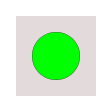
\includegraphics[width=\textwidth,keepaspectratio]{./040-komponenten/010-hardware/led-green.png}
    \caption{\label{fig:led-green}}
  \end{subfigure}
  \hspace{0.03\textwidth}
  \begin{subfigure}[b]{0.06\textwidth}
    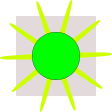
\includegraphics[width=\textwidth,keepaspectratio]
                    {./040-komponenten/010-hardware/led-green-blink.png}
    \caption{\label{fig:led-green-blink}}
  \end{subfigure}
  \hspace{0.03\textwidth}
  \begin{subfigure}[b]{0.06\textwidth}
    
\includegraphics[width=\textwidth,keepaspectratio]
                    {./040-komponenten/010-hardware/led-red-blink.png}
    \caption{\label{fig:led-red-blink}}
  \end{subfigure}
  \hspace{0.03\textwidth}
  \begin{subfigure}[b]{0.06\textwidth}
    
\includegraphics[width=\textwidth,keepaspectratio]{./040-komponenten/010-hardware/led-red.png}
    \caption{\label{fig:led-red}}
  \end{subfigure}
  \hspace{0.03\textwidth}
  \begin{subfigure}[b]{0.06\textwidth}
    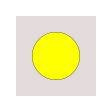
\includegraphics[width=\textwidth,keepaspectratio]
                    {./040-komponenten/010-hardware/led-yellow.png}
    \caption{\label{fig:led-yellow}}
  \end{subfigure}
  \hspace{0.03\textwidth}
  \begin{subfigure}[b]{0.06\textwidth}
    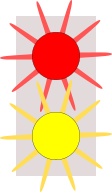
\includegraphics[width=\textwidth,keepaspectratio]
                    {./040-komponenten/010-hardware/led-red-yellow-blink.png}
    \caption{\label{fig:led-red-yellow-blink}}
  \end{subfigure}
  \caption{LED-Zustände \\ \small
           \textbf{(\subref*{fig:led-init})} Initialer Zustand
           \textbf{(\subref*{fig:led-start})} Spielstart
           \textbf{(\subref*{fig:led-green})} Spiel läuft
           \textbf{(\subref*{fig:led-green-blink})} Spielende naht \\
           \textbf{(\subref*{fig:led-red-blink})} wurde getroffen (unverwundbar)
           \textbf{(\subref*{fig:led-red})} tot
           \textbf{(\subref*{fig:led-yellow})} hat getroffen
           \textbf{(\subref*{fig:led-red-yellow-blink})} „letztes Leben“}
  \label{fig:leds}
\end{figure}
Jedes Spielgerät hat jeweils eine rote, eine gelbe und eine grüne LED, die wie auf einer Ampel
angeordnet sind.
Für Menschen mit Rot-Grün-Schwäche könnte man auch Prototypen bauen, bei denen die grüne LED durch
eine blaue LED ersetzt wird.
Mit diesen LEDs werden die verschiedenen Ereignisse kodiert.
Läuft kein Spiel und ist auch kein Spiel angekündigt, so leuchten alle LEDs der Reihe nach auf.
Dadurch können defekte, sowie nicht- oder falsch-angeschlossene LEDs schon direkt nach dem
Einschalten der Spielgeräte erkannt werden.
Wird ein Spiel angekündigt, so fangen alle LEDs synchron an zu blinken.
10 Sekunden vor dem Spielstart blinkt dann nur noch die rote LED und 4 Sekunden davor schalten die
LEDs, analog zu einer deutschen Straßenverkehrsampel, von rot über rot-gelb auf grün.
Die grüne LED zeigt an, dass das Spiel läuft.
Dies mag zwar kompliziert klingen, ist aber doch sehr intuitiv, denn solange die grüne LED nicht
leuchtet, weiß jeder, dass das Spiel noch nicht läuft, und wenn nach rot rot-gelb kommt, weiß jeder
aus Erfahrung, dass als nächstes grün kommt.

Neigt sich das Spiel dem Ende zu, fängt die grüne LED 64 Sekunden vorher langsam an zu blinken und
blinkt bis zum Ende des Spiels immer schneller.
Dies ist natürlich nur dann der Fall, wenn der Zeitpunkt des Spielendes vorher feststeht.
Nach dem Spielende kehren die LEDs zum initialen Zustand zurück.
Wenn das Spiel läuft, zeigt das Blinken der roten LED an, dass man getroffen wurde und unverwundbar
ist.
Auch sie wird immer schneller, wenn die Zeit der Unverwundbarkeit abläuft.
Zeigt die LED Dauerrot, dann ist man tot.
In diesem Zustand ist es auch nicht mehr möglich, andere Spieler abzuschießen, d.h. der IR-Sender
wird deaktiviert.
Die gelbe LED zeigt an, dass man einen anderen Spieler getroffen hat.
Das „letzte Leben“ wird dadurch angezeigt, dass die rote und die gelbe LED etwa alle 2 Sekunden für
100 Millisekunden synchron aufleuchten.
Hierbei ist anzumerken, dass es das Konzept von „Leben“ im übertragenen Sinne nur im Spielmodus
„No Carry No Win“ in Form von Dateifragmenten gibt, wie es im \cref{sec:spielmodi-speziell}
beschrieben wird.
In Spielmodi, in denen Spieler kein „letztes Leben“ haben können, wird dieser LED-Zustand nicht
genutzt.
Alle möglichen LED-Zustände sind zur Übersicht auch in \cref{fig:leds} dargestellt.

Ursprünglich wollten wir anstelle von LEDs ganze Displays verwenden, um auch individuelle
Informationen als Text oder eine Karte des Spielfeldes mit allen Mitspielern anzeigen zu können.
Neben des begrenzten Budgets und der Tatsache, dass Informationen dieser Art auch auf der Webseite
angezeigt werden können, war auch die begrenzte Zeit ein Grund dafür, dass wir diese Idee verworfen
haben.
Auch die Karte wurde nicht umgesetzt, da für die zuverlässige und genaue Positionsermittlung eines
Spielers in geschlossenen Räumen diverse Probleme zeit- und kostenintensiv gelöst werden müssten und
dies jenseits unserer Möglichkeiten in diesem Projekt gewesen wäre.
(Trotzdem wurde zunächst viel Zeit in diese Idee investiert.)
